\documentclass[russian,14pt]{eskdtext}
\usepackage[numbertop, numbercenter]{eskdplain}
\usepackage[utf8x]{inputenc}

\usepackage{setspace}
\onehalfspacing % полуторный интервал для всего текста

% - Подключаем шрифты из пакета scalable-cyrfonts-tex
\usepackage{cyrtimes}

% - Отступ красной строки
\setlength{\parindent}{1.25cm}

% - Убирает точку в списке литературы
\makeatletter
\def\@biblabel#1{#1 }

% ограничение для оглавления
%\usepackage{tocvsec2}
\setcounter{tocdepth}{2}

% - Точки для всех пунктов в оглавлении
\renewcommand*{\l@section}{\@dottedtocline{1}{1.5em}{2.3em}}
\renewcommand*{\l@subsection}{\@dottedtocline{1}{1.5em}{2.3em}}
%\renewcommand*{\l@subsubsection}{\@dottedtocline{1}{1.5em}{2.3em}}

% - Для переопределения списков
\renewcommand{\theenumi}{\arabic{enumi}}
\renewcommand{\labelenumi}{\theenumi)}
\makeatother

\usepackage{enumitem}
\setlist{nolistsep, itemsep=0.3cm,parsep=0pt}

% - ГОСТ списка литературы
\bibliographystyle{gost71u2003}

% - Верикальные отступы заголовков 
\ESKDsectSkip{section}{1em}{1em}
\ESKDsectSkip{subsection}{1em}{1em}
\ESKDsectSkip{subsubsection}{1em}{1em}

% - Изменение заголовков
\usepackage{titlesec}
\titleformat{\section}{\normalfont\normalsize\centering}{\thesection}{1.0em}{}
\titleformat{\subsection}{\normalfont\normalsize\centering}{\thesubsection}{1.0em}{}
\titleformat{\subsubsection}{\normalfont\normalsize\centering}{\thesubsubsection}{1.0em}{}
\titleformat{\paragraph}{\normalfont\normalsize\centering}{\theparagraph}{1.0em}{}

% - Оставим место под ТЗ 
%\setcounter{page}{4}

% - Для больших таблиц
\usepackage{longtable}
\usepackage{tabularx}
\renewcommand{\thetable}{\thesection.\arabic{table}}

% - Используем графику в документе
\usepackage{graphicx}
\graphicspath{{images/}}
\renewcommand{\thefigure}{\thesection.\arabic{figure}}

% - Счётчики
\usepackage{eskdtotal}

% - Выравнивание по ширине
\sloppy

% - Разрешить перенос двух последних букв слова
\righthyphenmin=2

% - Оформление списков
\RequirePackage{enumitem}
\renewcommand{\alph}[1]{\asbuk{#1}}
\setlist{nolistsep}
\setitemize[1]{label=--, fullwidth, itemindent=\parindent, 
  listparindent=\parindent}% для дефисного списка
\setitemize[2]{label=--, fullwidth, itemindent=\parindent, 
  listparindent=\parindent, leftmargin=\parindent}
\setenumerate[1]{label=\arabic*), fullwidth, itemindent=\parindent, 
  listparindent=\parindent}% для нумерованного списка
\setenumerate[2]{label=\alph*), fullwidth, itemindent=\parindent, 
  listparindent=\parindent, leftmargin=\parindent}% для списка 2-ой ступени, который будет нумероваться а), б) и т.д.
  
% - Оформляем листинг кода (не использовать комментарии на русском!)
\usepackage{listings}  
\lstset{basicstyle=\ttfamily\scriptsize}
\lstset{extendedchars=\true}

% - выводим текст как есть с размером шрифта scriptsize
\makeatletter
\def\verbatim{\scriptsize\@verbatim \frenchspacing\@vobeyspaces \@xverbatim}
\makeatother

% - Вставка pdf
\usepackage{pdfpages}

%межстрочный интервал
\usepackage{setspace}
\linespread{1.5}

\begin{document}
 \newpage
\ESKDthisStyle{empty}

\begin{center}
Министерство образования и науки Российской Федерации\\
Федеральное государственное бюджетное образовательное учреждение высшего профессионального образования\\
ТОМСКИЙ ГОСУДАРСТВЕННЫЙ УНИВЕРСИТЕТ СИСТЕМ УПРАВЛЕНИЯ И РАДИОЭЛЕКТРОНИКИ (ТУСУР)\\
Кафедра комплексной информационной безопасности электронно-вычислительных систем (КИБЭВС)\\
\end{center}

\vspace{2cm}

\begin{center}
Отчет по преддипломной практике \\
на тему \\
``Выбор протокола взаимодействия между датчиками и центральным сервером АСКУЭ''
\end{center}

\vspace{2cm}

\begin{flushright}
Выполнил: \\
студент гр. 720-1 \\
\underline{\hspace{2.5cm}}Д.С. Никифоров \\
"\underline{\hspace{1cm}}"\underline{\hspace{3cm}} 2015г.\\
\end{flushright}

\begin{flushright}
Утвердил: \\
Доцент каф.КИБЭВС \\
\underline{\hspace{2.5cm}}А.А. Конев \\
"\underline{\hspace{1cm}}"\underline{\hspace{3cm}} 2015г.\\
\end{flushright}

\vfill
\begin{center}
Томск -- 2015
\end{center}
 \newpage
\ESKDthisStyle{empty}
\paragraph*{\hfill РЕФЕРАТ \hfill}
Отчет по преддипломной практике содержит \ESKDtotal{page} страниц, \ESKDtotal{figure} рисунков,  6 таблиц, 3 источника.

АСКУЭ, ПРОТОКОЛ, СВЯЗЬ, СЕРВЕР, TCP/IP, QT, СЕТЬ, SQLITE.

Цель работы -- создание протокола взаимодействия между сервером и устройствами сбора данных АСКУЭ.

В ходе работы был сделан обзор существующих протоколов; реализована программа, эмулирующая функцию приема/передачи данных УСПД; реализована программа, осуществляющая взаимодействие с эмулятором и сохраняющая данный от эмулятора в базу данных.

Пояснительная записка выполнена при помощи системы компьютерной вёрстки \LaTeX.
 \newpage
\ESKDthisStyle{empty}

\begin{center}
Министерство образования и науки Российской Федерации\\
Федеральное государственное бюджетное образовательное учреждение высшего профессионального образования\\
ТОМСКИЙ ГОСУДАРСТВЕННЫЙ УНИВЕРСИТЕТ СИСТЕМ УПРАВЛЕНИЯ И РАДИОЭЛЕКТРОНИКИ (ТУСУР)\\
Кафедра комплексной информационной безопасности электронно-вычислительных систем (КИБЭВС)\\
\end{center}

\begin{flushright}
 \begin{minipage}{0.4\textwidth}
  УТВЕРЖДАЮ \\
  Зав. кафедры КИБЭВС \\
  \underline{\hspace{2.5cm}}А.А. Шелупанов \\
  "\underline{\hspace{1cm}}"\underline{\hspace{3cm}} 2015г.
 \end{minipage}
\end{flushright}

\vspace{2cm}

\begin{center}
 ЗАДАНИЕ \\
% На преддипломную практику
\end{center}

Студенту Дмитрию Сергеевичу Никифорову группы 720-1, факультета безопасности.

% 1. Тема преддипломной практики: ``Механизм взаимодействия датчиков и центрального сервера АСКУЭ''
% 
% 2. Исходные данные к проекту: Документация к проекту разработки АСКУЭ.
% 
% Руководитель практики: \\ директор ЦСП ТУСУР Антон Александрович Конев. 
% 
% \hfill Подпись руководителя: \underline{\hspace{2.5cm}}
% 
% \hfill "\underline{\hspace{1cm}}"\underline{\hspace{3cm}} 2015г.
% 
% Задание принял к исполнению
% 
% Студент гр. 720-1 Дмитрий Сергеевич Никифоров \hfill \underline{\hspace{2.5cm}}
% 
% \hfill "\underline{\hspace{1cm}}"\underline{\hspace{3cm}} 2015г.
 \newpage
 \tableofcontents
 \newpage
\section{Введение}
\setcounter{figure}{0}

%Целью данной работы является определить наиболее популярные протоколы передачи данных, поддерживаемые в приборах и системах учета, с целью их анализа, выбора и дальнейшей реализации в разрабатываемой автоматизированной системе коммерческого учета энергоресурсов, 

Целью данной работы является создание протокола взаимодействия между сервером сбора данных (ССД) и устройствами съема и передачи данных(УСПД) в автоматизированной системе коммерческого учета энергоресурсов (АСКУЭ).

Создание нового протокола необходимо для использования АСКУЭ в сфере ЖКУ, так как существующие протоколы ориентированы на использования в пределах предпприятий, из-за чего существующие протоколы не учитывают аспекты информационной безопасности, в протоколах отсуствует авторизация, линии связи обладают недостаточно дальностью передачи сигнала без использования повторителей. 

Всё это приводит к серьезным проблемам при использвании АСКУЭ в условиях ЖКУ. Появляется проблема передачи данных от УСПД до ССД, так как для использования существующих протоколов необходимо прокладывать линии связи. Использование протоколов так же не гарантиреут подлиности и аутентичность передаваемых данных. 

%После чего необходимо реализовать функции взаимодействия сервера с устройством съема и передачи данных (УСПД) по данному протоколу, в том числе разработать систему команд взаимодействия с УСПД.
 \newpage
\section{Протоколы обмена данными в автоматизированных системах контроля}
\setcounter{figure}{0}

На рынке представлено множество датчиков, которые связываются с системой по различным протоколам. Используются такие протоколы как \cite{csp}:
\begin{itemize}
\item TCP/IP;
\item Modbus;
\item Canbus;
\item МЭК 60870-5-101;
\item МЭК 60870-5-104;
\item ОРС;
\item "Пирамида" (закрытый протокол);
\item спецпротоколы электросчетчиков;
\item SNMP;
\item TFTP;
\item RTU-325.
\end{itemize}

\subsection{Стандарт OPC}

OPC (OLE for Process Control) – семейство протоколов, предоставляющих единый интерфейс для управления объектами автоматизации и технологическими процессами. В частности, OPC DA (DataAccess) — стандарт, описывающий набор функций обмена данными в реальном времени с объектами автоматизации. 

Спецификация OPC охватывает:
\begin{itemize}
 \item концепцию клиент-серверную технологию OPC и определение данных;
 \item описания интерфейсов, методов, параметров и возможное их поведение;
 \item описание типов и структур данных;
 \item общие виды деятельности, которые включают в себя определение адресного пространства и его просмотра. Чтение, запись и подписка на уведомления об обновлении данных.
\end{itemize}

К недостаткам этого OPC можно отнести:
\begin{itemize}
 \item необходимость платного членства в сообществе The InteroperabilityStandard for Industrial Automation;
 \item протокол основан на технологиях windows.
\end{itemize}

Данный протокол не подходит, так как для его использования необходимо платное членство, что является неприемлемым для заказчика.

\subsection{Стандарт МЭК-60870-5-101/104}

МЭК-60870-5-101/104 – это протокол передачи данных, применяется в АСКТУ, АСКУЭ. Особенности реализации протокола МЭК 60870-101/104 при передаче данных между объектом и диспетчерским центром:

\begin{itemize}
 \item передача ограниченного количества информации, что обусловлено необходимостью переназначения всех сигналов с одного протокола на другой, и, как следствие, потеря некоторых данных, передача которых на этапе проектирования не была сочтена целесообразной;
 \item отсутствие единых наименований сигналов в рамках объекта и в центрах управления сетями, приводящее к сложности наладки и отслеживания ошибок;
 \item протокол МЭК 60870-5-101 предназначен для передачи данных по последовательным линиям связи RS-232/485;
 \item протокол МЭК 60870-5-104 является расширением протокола 101 и регламентирует использование сетевого доступа по протоколу TCP/IP.
\end{itemize}

Недостатки реализации данного стандарта:

\begin{itemize}
 \item количество передаваемых сигналов ограничивается определенным количеством дискретных входов и выходов;
 \item отсутствует возможность контроля связи между устройствами;
 \item возможно ложное срабатывание дискретного входа устройства при замыкании на землю в цепи передачи сигнала;
 \item цепи подвержены воздействию электромагнитных помех;
 \item сложность расширения систем;
 \item передача данных осуществляется в два этапа:
 \begin{enumerate}
  \item назначение индексированных коммуникационных объектов на прикладные объекты;
  \item  назначение прикладных объектов на переменные в прикладной базе данных или программе. Таким образом, отсутствует семантическая связь (полностью или частично) между передаваемыми данными и объектами данных прикладных функций.
 \end{enumerate}
 \item протоколы не предусматривают возможность передачи сигналов реального времени.
\end{itemize}

Данный протокол не подходит ввиду ограниченности возможностей и сложности масштабирования системы.

\subsection{Стандарт MODBUS}

Modbus – один из наиболее распространенных сетевых протоколов для интеграции устройств РЗА (релейная защита автоматики) в систему АСТУ, построенный на архитектуре «клиент–сервер». Данный протокол является открытым, что частично обуславливает его популярность. Протокол Modbus для передачи данных использует такие линиям связи как RS-485, RS-433, RS-232, а также сети TCP/IP (Modbus TCP).

Стандарт Modbus содержит в себе:

\begin{itemize}
 \item спецификация прикладного уровня;
 \item спецификация канального уровня;
 \item спецификация физического уровня;
 \item спецификацию ADU для транспорта через стек TCP/IP.
\end{itemize}

К достоинствам стандарта относится:

\begin{itemize}
 \item массовость;
 \item относительная простота реализации систем на его базе.
\end{itemize}

К недостаткам данного протокола можно отнести:

\begin{itemize}
 \item в случае необходимости отсутствует возможность оперативной сигнализации от конечного устройства к мастеру;
 \item стандарт не регламентирует начальную инициализацию системы. Назначение сетевых адресов и параметров системы для каждого устройства выполняются вручную на этапе адаптации;
 \item отсутствие  возможности  конечным  устройствам  обмениваться фиксированными данными друг с другом без участия мастера. Что ограничивает  применимость MODBUS-решений в системах регулирования реального времени.
\end{itemize}

Данный протокол не подходит ввиду отсутствия возможности оперативной сигнализации от конечного устройства к мастеру.

\subsection{Стандарт CAN}

CAN (Controller Area Network) – стандарт промышленной сети, использующийся для объединения в единую сеть устройств и датчиков. Применяется в системах автоматизации промышленного производства. 

В первую очередь данный стандарт описывает физический уровень, наибольшую популярность получил вариант описанный в ISO 11898-2. Физический уровень использует дифференциальную передачу данных по витой паре, для управления доступом к шине используется неразрушающее bit-wise разрешение конфликтов ISO 11898.

К положительным аспектам данной реализации относиться:

\begin{itemize}
 \item работа в режиме жёсткого реального времени;
 \item высокая устойчивость к помехам;
 \item надёжный контроль ошибок приема-передачи данных.
\end{itemize}

К достоинствам данного стандарта относятся:

\begin{itemize}
 \item сообщения имеют малые размеры (8 байт данных) и защищены контрольной суммой;
 \item большой размер служебных данных в пакете по отношению к полезным данным;
 \item отсутствие единого общепринятого стандарта на протокол высокого уровня (в том числе TCP).
\end{itemize}

Данный протокол не подходит из-за сложностей использования в сетях интернет.

\subsection{Стандарт DLMS}

DLMS (Device Language Message Specification) – стек протоколов, ориентированный на 16-разрядные микроконтроллеры Microchip PIC. Является международным стандартом для систем сбора данных с электро-, газовых, водяных и тепловых счетчиков. Работает на основе протоколов связи (RS232, RS485, PSTN, GSM, GPRS, IPv4, PPP и PLC), с поддержкой шифрования AES128.

Особенности данного протокола:

\begin{itemize}
 \item работает на всех 16-битных микроконтроллерах PIC и dsPIC;
 \item возможность интеграции стека DLMS с текущими реализациями протоколов TCP/IP, ZigBee и PLC;
 \item небольшой объем занимаемой памяти позволяет использовать компактные и недорогие контроллеры;
 \item для европейского рынка стек поддерживает IEC 62056-21 Mode E.
\end{itemize}

К недостаткам данного протокола можно отнести то, что описание протокола предоставляется на платной основе или требуется членство в ассоциации DLMS. Что является неприемлемым для заказчика.

Из представленного краткого анализа видно, что существующие протоколы связи достаточно успешно позволяют реализовывать задачи диспетчерского управления / интеграции данных в системы управления, однако не все они позволяют реализовывать функции реального времени. К тому же большое количество проприетарных протоколов приводит к усложнению процесса интеграции устройств в единую систему: 

\begin{itemize}
 \item протоколы должны поддерживаться контроллером, что требует реализации поддержки большого количества протоколов в в нем и ведет к удорожанию оборудования;
 \item для интеграции устройств по проприетарным протоколам требуется квалификация наладочного персонала в работе с каждым из них;
 \item переназначение сигналов из проприетарных протоколов в общепромышленные и назад часто приводит к потере информации, включая дополнительную информацию;
 \item при передаче данных по-прежнему применяется большое количество последовательных интерфейсов, что накладывает ограничения на скорость передачи данных, объем передаваемых данных и количество устройств, одновременно включенных в информационную сеть.
\end{itemize}

\subsection{Предлагаемое решение}

Большинство приборов учета (или УСПД) поддерживают протокол передачи данных TCP/IP, в виду чего использование данного протокола на транспортном уровне является целесообразным, так как в отличие от других протоколов передачи данных TCP/IP имеет следующие преимущества:

\begin{itemize}
 \item скорость разработки и цена разработки;
 \item использование в сетях интернет;
 \item более простой (простая поддержка);
 \item обеспечивает контроль целостности передаваемых данных;
 \item возможность обеспечить программную поддержку новых устройств через модульную систему драйверов.
\end{itemize}

TCP (англ. Transmission Control Protocol, протокол управления передачей) — один из основных протоколов передачи данных Интернета, предназначенный для управления передачей данных в сетях и подсетях TCP/IP\cite{tcp}.

Для обеспечения защищенного соединения необходимо использовать технологии построения виртуальных каналов. 

Технология построения защищенного соединения в открытых сетях так же позволит решить проблему конфиденциальности передаваемых данных благодаря тому, что весь передаваемый трафик передается в шифрованном виде. Примером таких технологий является технология VPN. VPN (англ. Virtual Private Network — виртуальная частная сеть\cite{vpn}) — обобщённое название технологий, позволяющих обеспечить одно или несколько сетевых соединений (логическую сеть) поверх другой сети (например, Интернет). Несмотря на то, что коммуникации осуществляются по сетям с меньшим или неизвестным уровнем доверия (например, по публичным сетям), уровень доверия к построенной логической сети не зависит от уровня доверия к базовым сетям благодаря использованию средств криптографии (шифрования, аутентификации, инфраструктуры открытых ключей, средств для защиты от повторов и изменений передаваемых по логической сети сообщений).

Так же для решения данной задачи возможно использование технологии SSH. SSH (англ. Secure Shell — «безопасная оболочка»\cite{ssh}) — сетевой протокол прикладного уровня, позволяющий производить удалённое управление операционной системой и туннелирование TCP-соединений (например, для передачи файлов). Схож по функциональности с протоколами Telnet и rlogin, но, в отличие от них, шифрует весь трафик, включая и передаваемые пароли. SSH допускает выбор различных алгоритмов шифрования. SSH-клиенты и SSH-серверы доступны для большинства сетевых операционных систем. 

Тогда последовательность действий при запросе данных от ССД к УСПД имеет следующий вид:

\begin{enumerate}
 \item установление соединения между ССД и УСПД;
 \item отправка идентификационных данных ССД на УСПД;
 \item отправка запроса на получение данных от УСПД;
 \item получение данных от УСПД;
 \item завершение соединения.
\end{enumerate}

Функциональная схема данного процесса представлена на рисунке \ref{img:get_data_idef0}.

\begin{figure}[!ht]
 \center{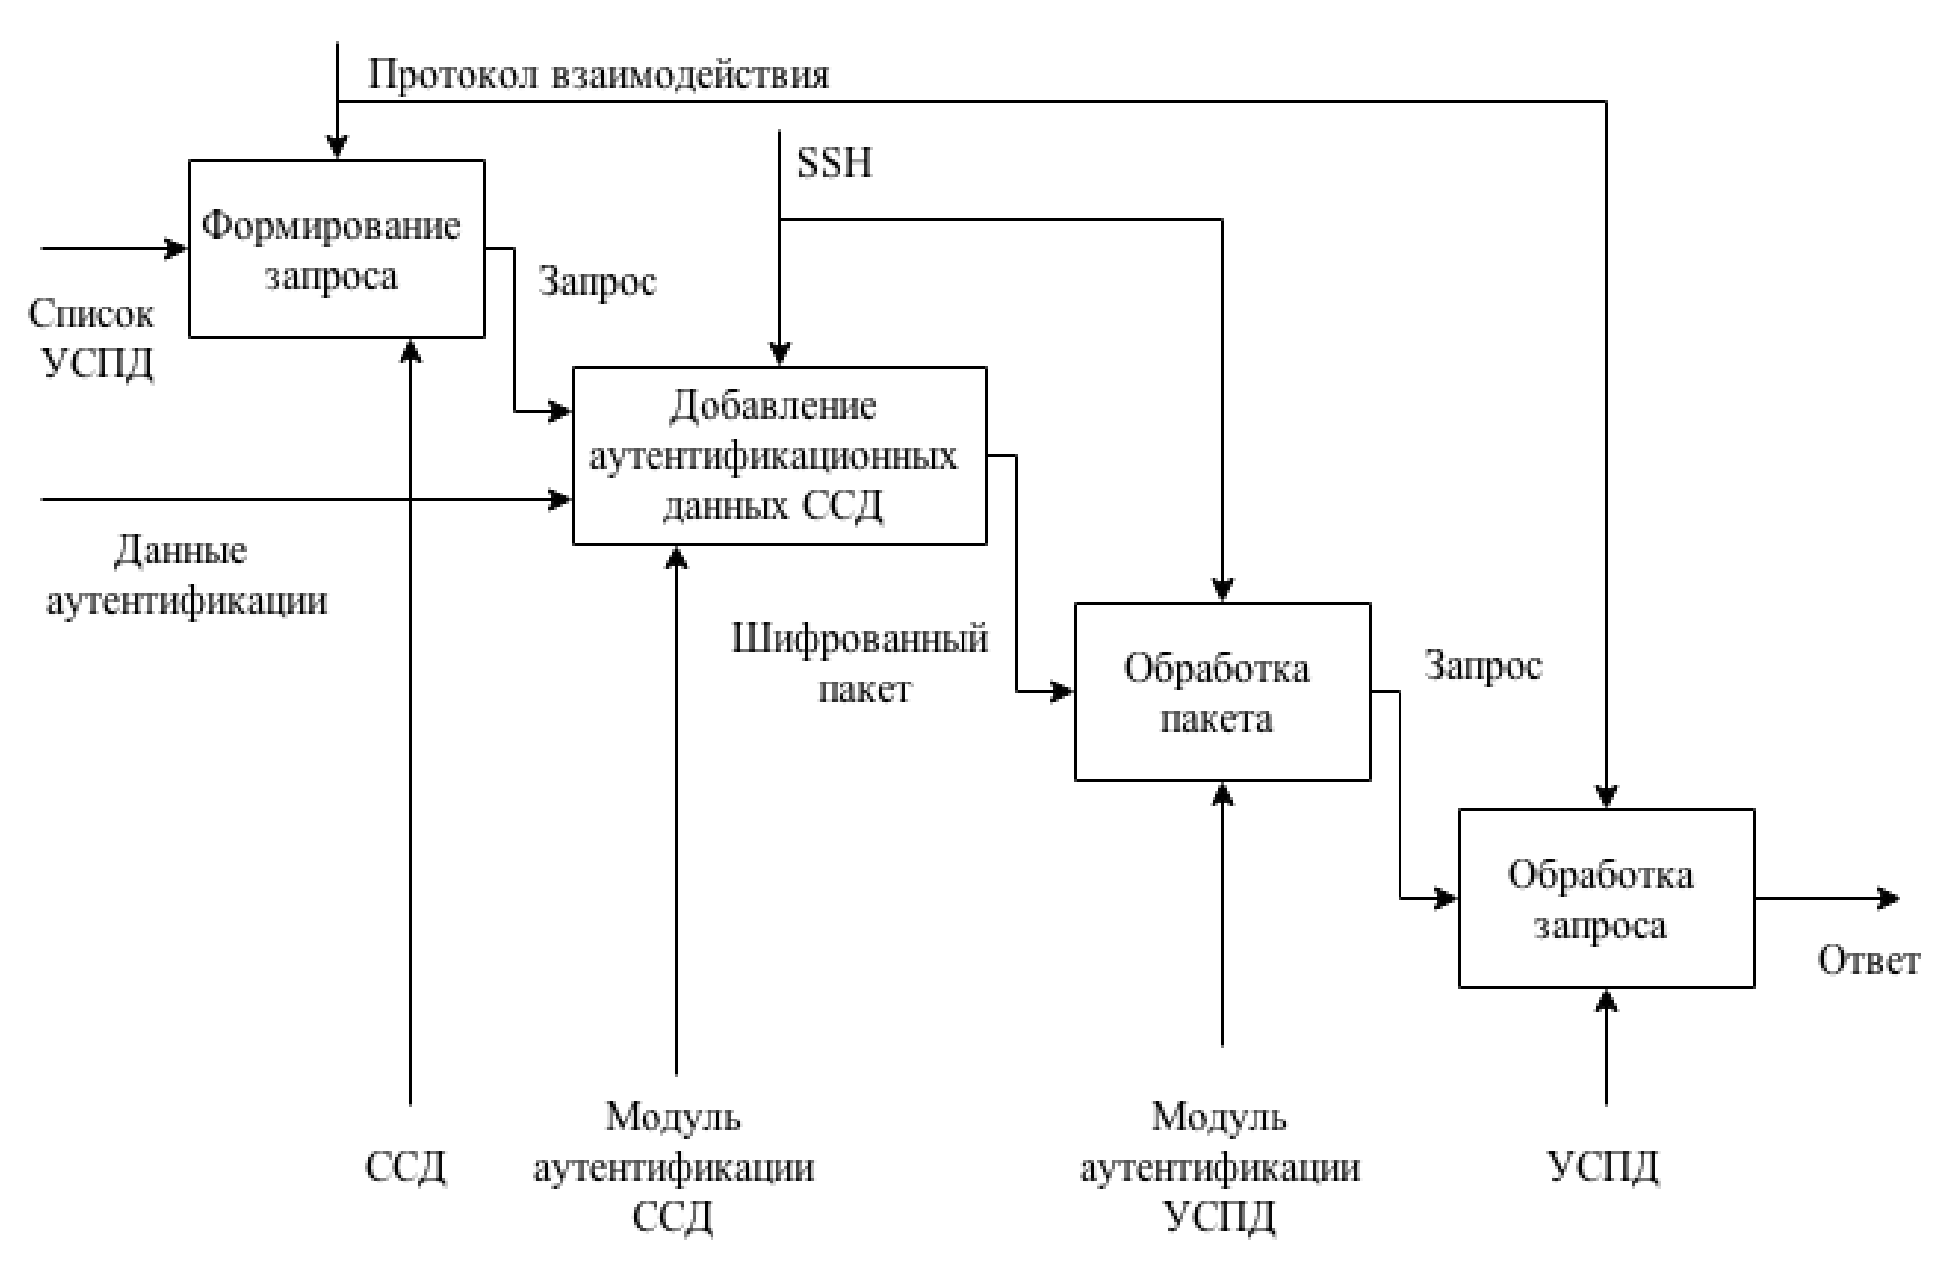
\includegraphics[width=0.8\linewidth]{get_data_idef0}}
 \caption{Запрос данных с УСПД}
 \label{img:get_data_idef0}
\end{figure}

Использование технологий построения виртуальных частных каналов позволяет защититься от угроз:

\begin{itemize}
 \item внедрение ложного объекта сети;
 \item анализ сетевого трафика;
 \item подмена доверенного объекта;
 \item навязывание ложного маршрута;
 \item выведывание паролей.
\end{itemize}

 \newpage
\section{Механизм взаимодействия сервера сбора данных с УСПД}
\setcounter{figure}{0}

В разрабатываемой системе сервер является инициатором всех обменов данными, а клиенты ожидают запроса для передачи данных. Схема взаимодействия приведена на рисунке \ref{scheme2:scheme2}.

\begin{figure}[h!]
 \center{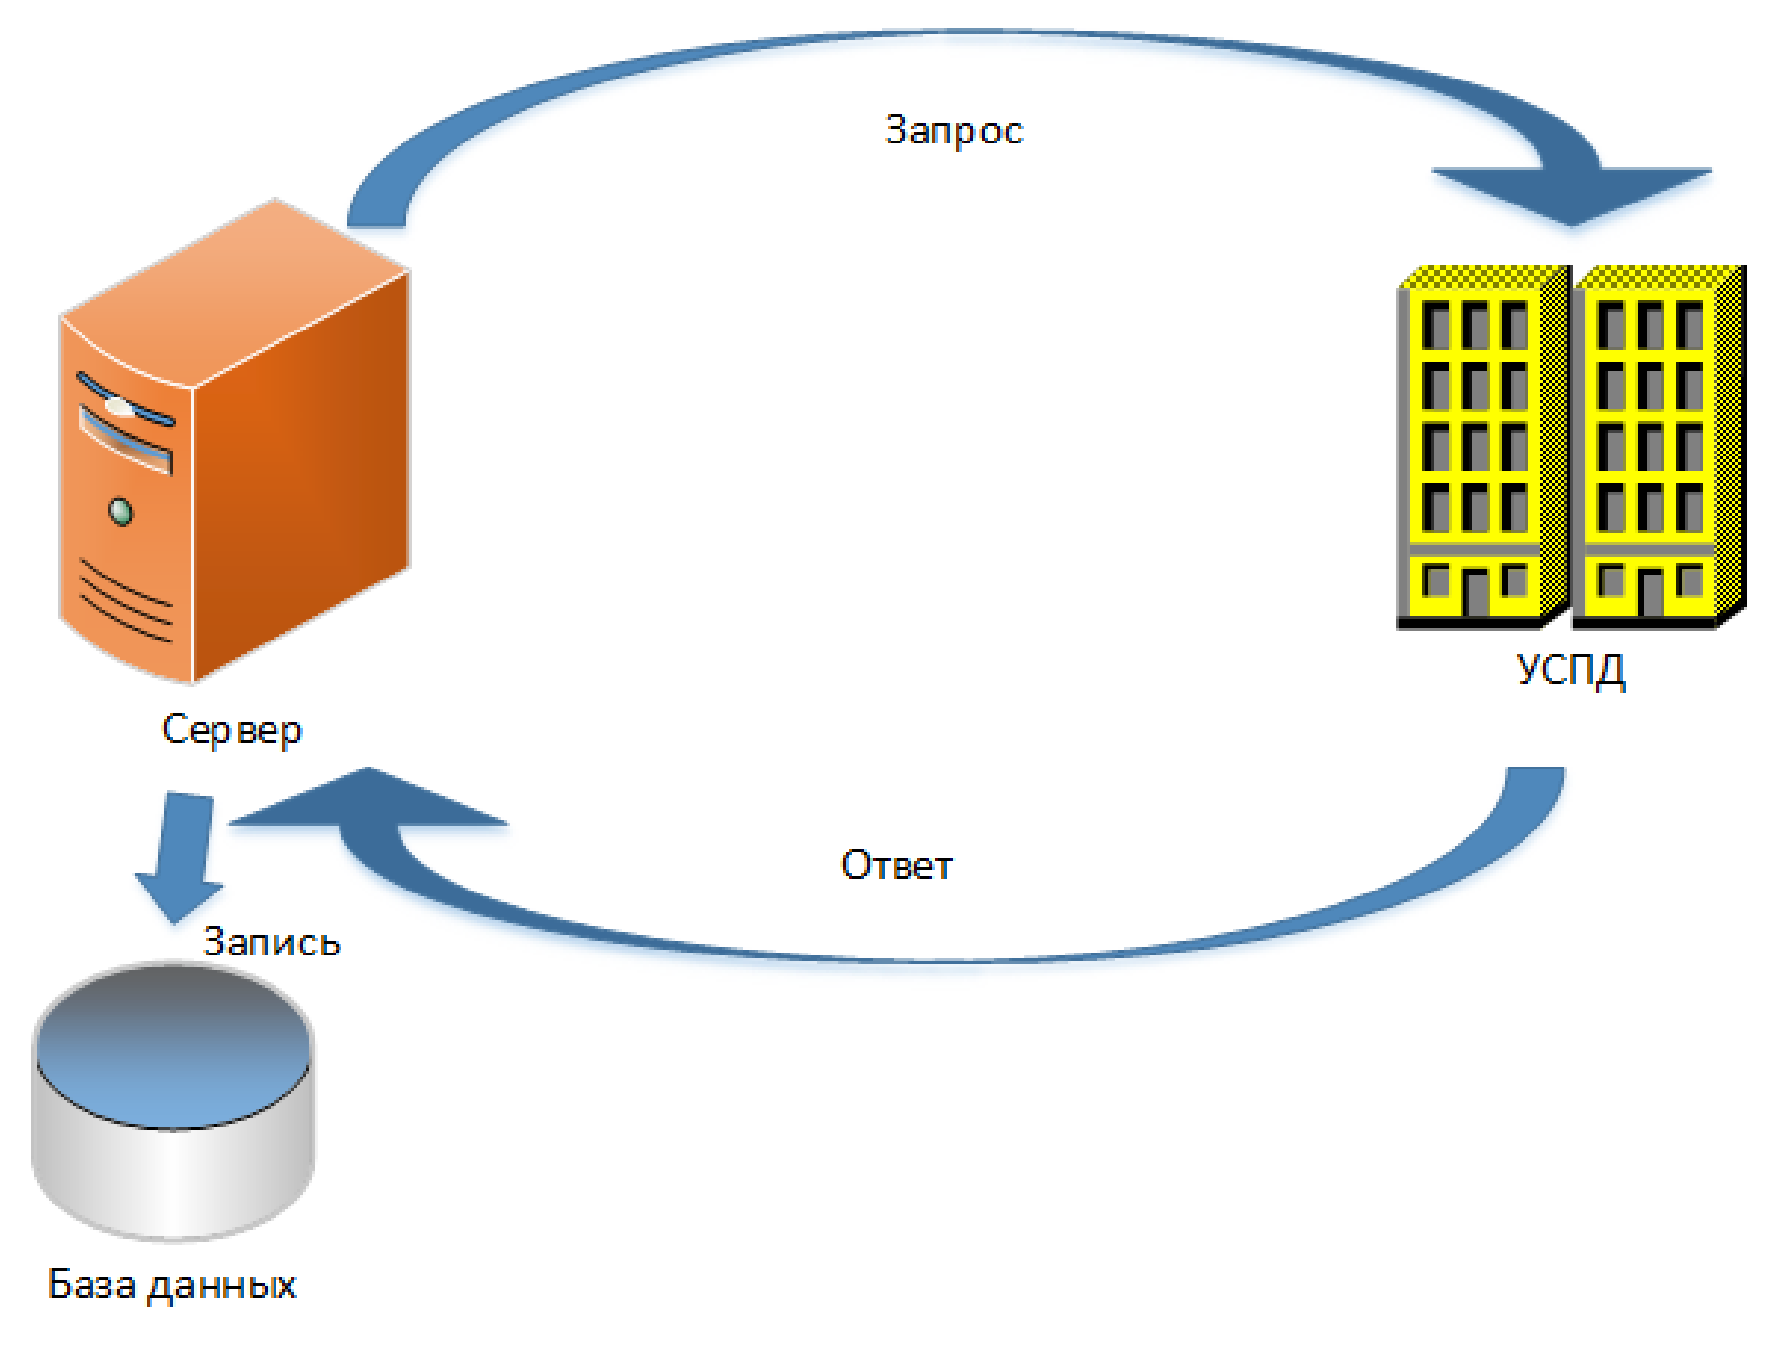
\includegraphics[width=0.8\linewidth]{scheme2}}
 \caption{Схема взаимодействия сервера с УСПД}
 \label{scheme2:scheme2}
\end{figure}

Данный механиз позволяет реализовать опрос УСПД по списку, хранящемуся на сервере, что исключит возможность отправки данных с несанкционированных устройств. Так же появляется возможность обнаружения неисправности УСПД либо ошибки сети, на который сервер будет реагировать предупреждениями. 

Данные, полученные с УСПД, записываются во временную базу данных для последующей обработки и отправки на центральный сервер. В этой же базе данных хранится список всех УСПД, подконтрольных данному серверу. Схема представлена на рисунке \ref{scheme3:scheme3}.

\begin{figure}[h!]
 \center{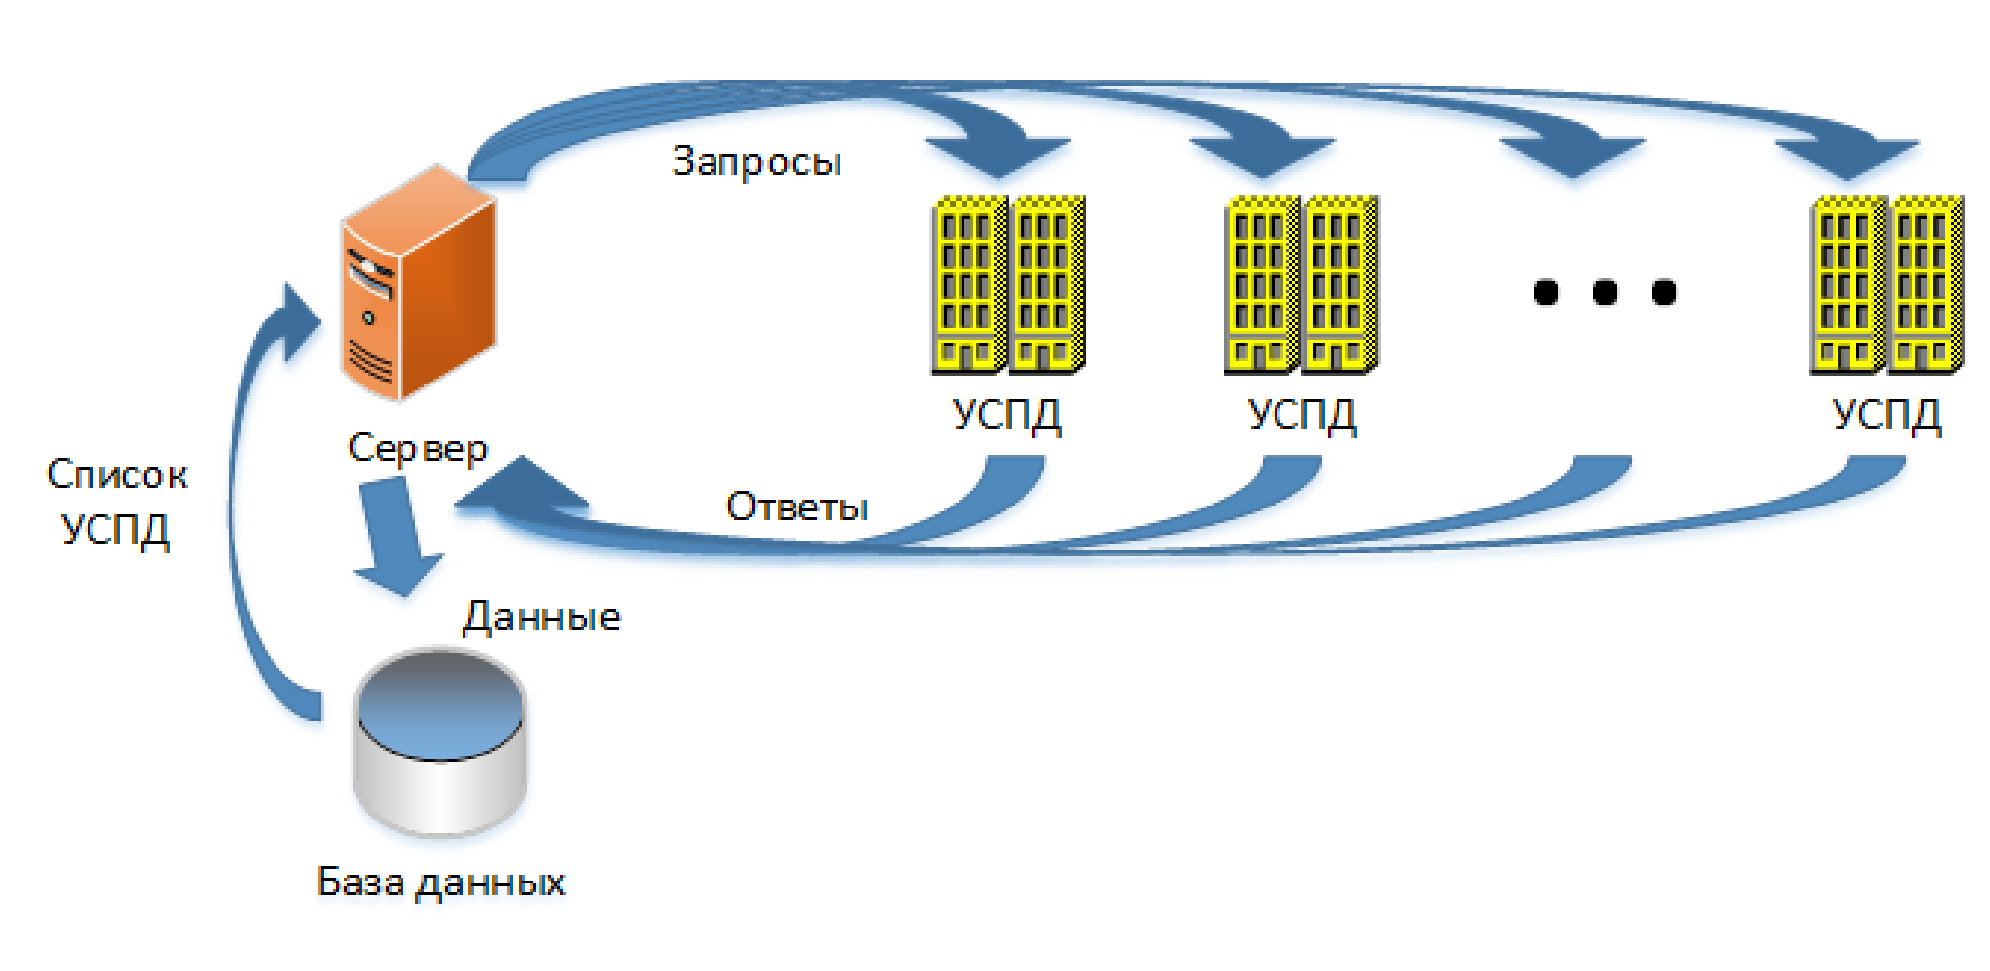
\includegraphics[width=0.8\linewidth]{scheme3}}
 \caption{Механизм взаимодействия с группой УСПД}
 \label{scheme3:scheme3}
\end{figure}

 \section{Сетевое взаимодействие}

Было принято решение реализовывать взаимодействие УСПД и центрального сервера по протоколу TCP/IP.

Механизм TCP предоставляет поток данных с предварительной установкой соединения, осуществляет повторный запрос данных в случае потери данных и устраняет дублирование при получении двух копий одного пакета, гарантируя тем самым целостность передаваемых данных и уведомление отправителя о результатах передачи.

\subsection{Сетевое взамодействие в Qt Framework}

Сетевое взаимодействие в программах, реализованных на языке C++ реализуется при помощи сокетов, в Qt для реализации данного взаимодействия используется надстройка над механизмом сокетов, облегчающая реализацию данного взаимодействия.

Данный механизм представлен такими классами как \cite{qt_net}:
\begin{itemize}
 \item QAbstrackSocket;
 \item QTcpSocket;
 \item QTcpServer;
 \item QUdpSocket.
\end{itemize}

Для реализации взаимодействия будут использоваться классы QTcpSocket и QTcpServer.

\subsection{УСПД}

Для тестирования разрабатываемой программы был сделан эмулятор, на базе одноплатного компьютера Raspberry Pi B+. 

Для данного компьютера был написан скрипт на языке python. Задачей скрипта является открыть порт на устройстве и реагировать на все данные, приходящие на этот порт отправкой данных в обратном порядке. 

Текст скрипта:

\begin{lstlisting}
#!/usr/bin/python
# -*- coding: utf-8 -*-

import socket

sock = socket.socket()
sock.bind(('', 9090))
sock.listen(5)
while True:
        conn, addr = sock.accept()
        while True:
                data = conn.recv(1024)
                if not data:
                        break
                buf = data[::-1] + '\n'
                print data
                conn.send(buf)

conn.close()
\end{lstlisting}

\subsection{Взаимодействие с УСПД}

В первую очередь необходимо реализовать функцию оптравки данных по сети. 

Для этого был создана программа с графическим итерфейсом. Задачей данной программы является установление соединения с определенным адресом и получением/отправкой текстовой информации.

Прототип объекта, решающего эту задачу, выглядит так:

\begin{lstlisting}
class EmulSocket : public QObject
{
    Q_OBJECT
public:
    explicit EmulSocket(QObject *parent = 0);
    ~EmulSocket();
    void configure(QString, int);
    void initSocket();
    void sendData(QByteArray);

private:
    QString qs_Address;
    int i_Port;
    QTcpSocket * sc;
signals:
    void haveData(QString);
public slots:
    QString getData();
};
\end{lstlisting}

В конструкторе и диструкторе объекта инициализируется и уничтожается объект QTcpSocket *sc.

Метод configure(QString, int) заполняет значения ip-адреса и порта назначения (поля qs\_Address и i\_Port соответственно), так же в данном методе происходит связывание события ``приняты данные'' с обработчиком этого события - методом getData(). После чего вызывается метод initSocket().

Метод initSocket() отвечает за установление соединения с указанным хостом.

Метод sendData(QByteArray) - это функция, отправляющая полученный массив байт по адресу назначения.

Сигнал haveData(QString) - это вспомогательный сигнал для взаимодействия объекта с графическим интерфейсом.

Метод getData() обрабатывает входящий поток данный и при получении данных испускает сигнал haveData(QString) в котором передает полученные данные.

Интерфейс программы представлен на рисунке \ref{window1:window1}.

\begin{figure}[h!]
 \center{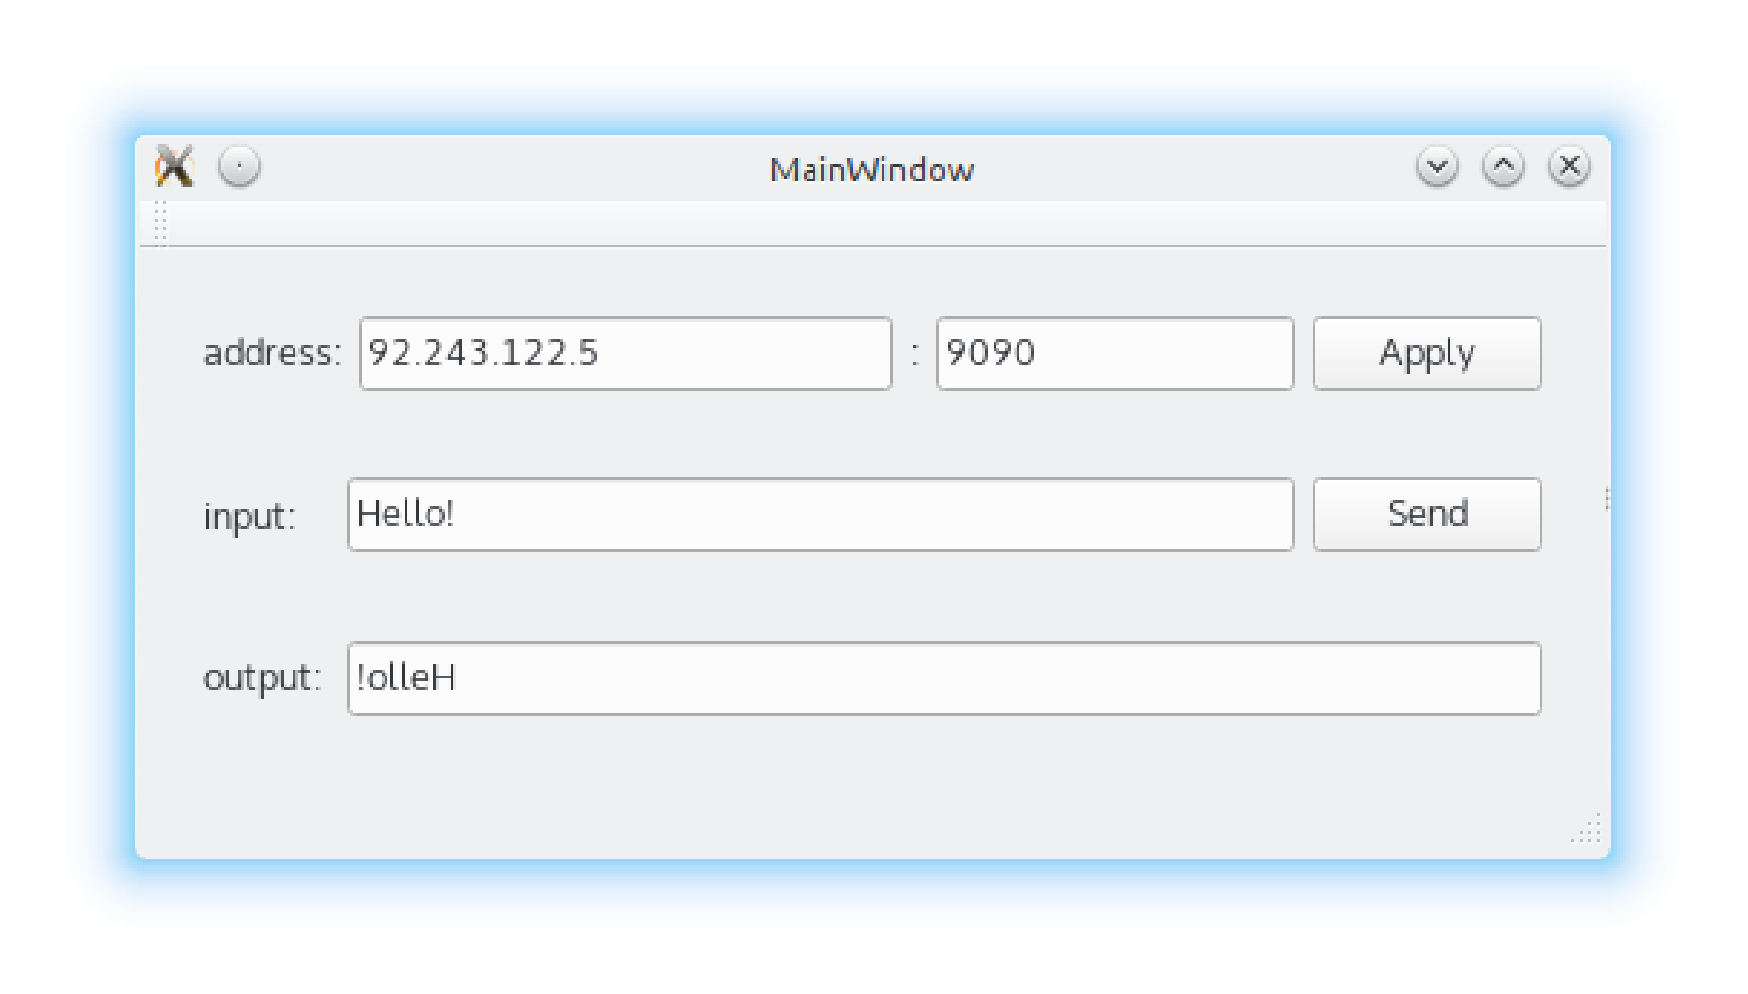
\includegraphics[width=0.7\linewidth]{window1}}
 \caption{Подключение к эмулятору УСПД}
 \label{window1:window1}
\end{figure}

\subsection{Сохранение данных}

После установления связи с УСПД необходимо фиксировать полученную информацию в базе данных. Для теста была выбрана СУБД SQLite. 

Необходимо записывать в базу данных все ответы с эмулятора, при этом дописывать к ним время получения.

В базе данных создана одна таблица с тремя полями: id, data, time.

Для реализации данного функционала необходимо реализовать функции для работы с базой данных. Для этого в реализованном ранее приложении был добавлен новый объект. 

Описание объекта:

\begin{lstlisting}
class EmulDB : public QObject
{
    Q_OBJECT
public:
    explicit EmulDB(QObject *parent = 0);
    ~EmulDB();

    bool dbConnect(const QString& );
    void dbDisconnect();
    bool dbInsert(const QString& );

private:
    QSqlDatabase m_db;
    bool m_bOpen;
};
\end{lstlisting}
Конструктор и диструктор не выполняют каких либо дополнительных действий, атрибуты m\_db и m\_bOpen это база данных и её состояние (подключена ли база данных) соответственно.

Методы dbConnect и dbDisconnect необходимы для подключения и отключения к базе даных. 

Метод dbInsert принимает данные и записывает их в таблицу, подставляя время записи.

На рисунке \ref{dBase:dBase} представлено содержимое базы данных после тестового запуска программы.

\begin{figure}[h!]
 \center{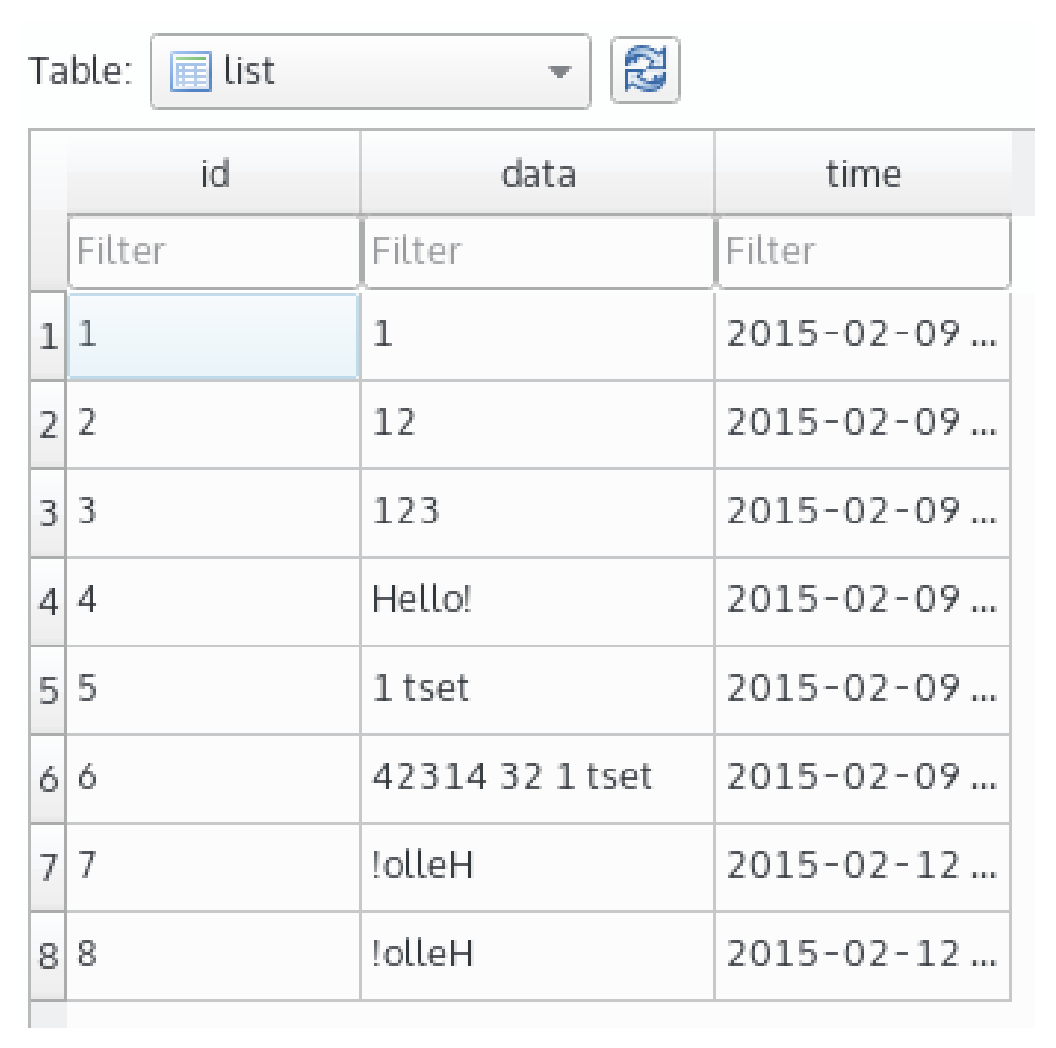
\includegraphics[width=0.7\linewidth]{dBase}}
 \caption{Просмотр таблицы}
 \label{dBase:dBase}
\end{figure}
 \section{Сервер сбора данных}
\subsection{Постановка задачи}

В первую очередь необходимо реализовать функции опроса клиентов. Так же программа должна обладать информацией о клиентах, тоесть иметь список данных клиентов, в которых содержится адрес клиента (ip-адрес и номер порта).

Так же для тестировани необходим более сложный эмулятор, который бы поддерживал несколько параллельный подключений с выводом информации о появлении нового подключения, разрыве соединения и отображения полученной информации.

\subsection{Приложение-клиент}

Так как это вспомогательное приложение, для простоты разработки не будем создавать для него графический интерфейс. 

Идея состоит в том, что бы создать приложение которо ожидает подключения и при появлении такового создает новое tcp соединение и принимает информацию, так же приложение должно проверять статус соединения и при его разрыве удалять созданные сокеты для освобождения портов. Данный механизм в дальнейшем будет использоваться и на сервере.

Для ожидания соединения нам нужно создать специальный объект, которы реагировал бы на обращение к определенному порту клиентской машины. Для создания такого объекта воспользуемся классом QTcpServer. Данный класс порождает объекты, которые, прослушивающие порт и испускающие сигналы при появлении запроса на соединение.

Создадим класс TestServ. Прототип класса представлен ниже.

\begin{lstlisting}
class TestServ : public QObject
{
    Q_OBJECT
public:
    explicit TestServ(QObject *parent = 0);
    ~TestServ();

    void initServ(const int &port);

private:
    QTcpServer *srv;
    QMap<QString, ClientSock*> users;
signals:

public slots:
    void newConnection();
    void connectClosed(QString name);
};
\end{lstlisting}
В конструкторе и диструктора класса инициилизируется объект srv, так же в конструкторе связывается сигнал объекта srv newConnection со слотом данного класса newConnection.

Метод initServ указывает объекту srv какой порт необходимо прослушивать, и выводит в консоль информацию о том, успешно ли прошел запуск сервера.

QMap<QString, ClientSock*> users - это контейнер для хранения указателей на созданные в даный момент сокеты с присвоенными им именами.

Слот newConnection() отрабатывает при появлении нового запроса на соединение, здесь в консоль выводится сообщение о создании нового запроса и создается и инициализируется объект ClientSock*, после чего его сигнал scDisconnect(QString) связывается со слотом connectClosed(QString) и указатель помещается в QMap.

Слот connectClosed принимает на вход имя слота, производит поиск укзателя с данным именем, отдает команду уничтожить объект и удаляет запись о данном объекте из QMap.

Объект ClientSock это ранее созданный класс EmulSock с добавлением нескольких методов и сигналов. Прототип данного класса представлен ниже.

\begin{lstlisting}
class ClientSock : public QObject
{
    Q_OBJECT
public:
    explicit ClientSock(QObject *parent = 0);
    explicit ClientSock(QTcpSocket *sock, QObject *parent = 0);
    ~ClientSock();
    void initSc(const QString & addr, const int & port);
    void setName(const QString & name);
    QString getName();
    void sendData(QByteArray data);
    void timerEvent(QTimerEvent *event);
private:
    QTcpSocket * sc;
    QString m_qsScName;
signals:
    void scDisconnect(QString);
public slots:
    QByteArray getData();
};
\end{lstlisting}

В описании добавился конструктор, принимающий указатель на объект QTcpSocket, необходимый для создания объекта на основании данных, полученных от объекта srv.

Методы getName и setName необходиы для работы с атрибутом m\_qsScName, хранящую имя объекта.

Метод timerEvent необходим для отслеживания статуса сокета sc, данный метод вызывается всякий раз при обнулении таймера, запускаемого при создании объекта типа ClientSock в констукторе. Данный метод проверяет статус сокета и при получении статуса ``отключен'' останавливате таймер, выводит сообщение о прекращении соединения и испускает сигнал что соединение закрыто, который обрабатывается объектом типа TestServ.

В функции main просто создаем объект типа TestServ, и указываем ему порт назначения, переданный первым аргументом при запуске программы. Пример работы с подключением одного клиента представлен на рисунку \ref{clientEmul:clientEmul}.

\begin{figure}[h!]
 \center{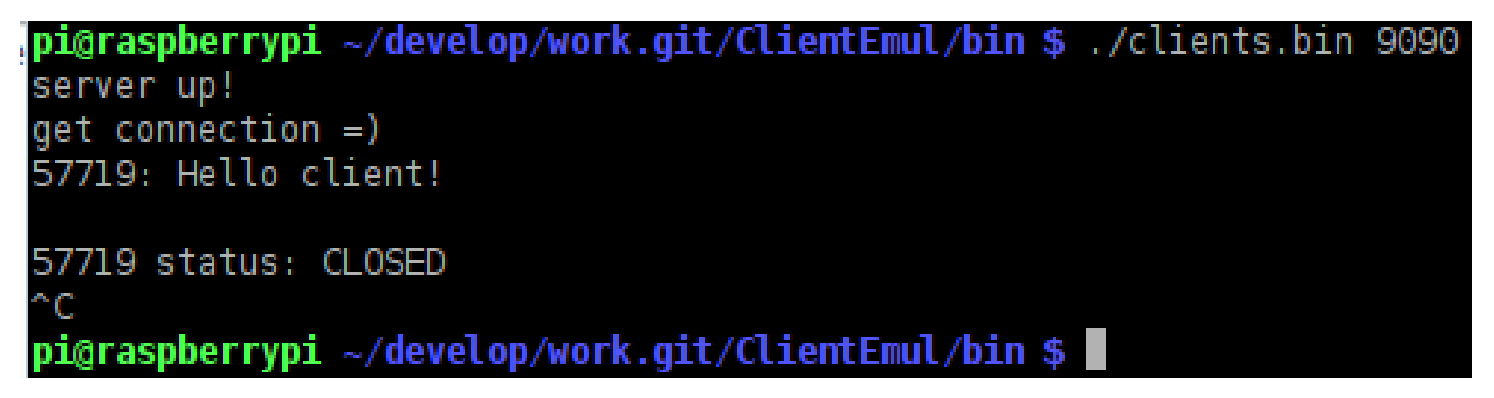
\includegraphics[width=0.7\linewidth]{clientEmul}}
 \caption{Демонстрация работы приложения}
 \label{clientEmul:clientEmul}
\end{figure}

 \newpage
 %TODO
 \newpage
\section{Заключение}
\setcounter{figure}{0}

В ходе выполнения данной работы были рассмотрены существующие протоколы обмена данными в системах автоматизированного контроля, сделан вывод о необходимости создания своего протокола обмена данными между УСПД и ССД так как существующие протоколы не отвечают требованиям системы. 

Разработана структура данных для пересылки показаний от УСПД на ССД, механизм опроса УСПД, а так же предложена система команд для управления УСПД.


Предложенное решение позволяет связывать УСПД и ССД через сеть интернет, осуществляет контроль целостности передаваемыз данных и обеспечивает конфиденциальность передаваемых данных при помощи шифрования.

Так же подсчитана экономическая эффективность проекта. По результатам подсчетов сделан вывод о целесообразности продолжения проекта. Использование системы для сбора показаний устройств учета снижает трудоемкость процесса сбора показаний с устройств учета на 80\%.
 
 \newpage
 \section*{Список использованных источников}
 \addcontentsline{toc}{section}{Список использованных источников}
 1. Энергосбережение: приборы учета // РБК Research. - 2013.
 
 2. Обзор и варианты построения архитектуры АСКУЭ // цсп ТУСУР. - 2014.
 
 3. Шлее, М. Qt 4.5: Профессиональное программирование на С++ / Макс Шлее. - СПб.: БХВ Петербург, 2010. - 896 с.
\end{document}

